%%%%%%%%%%%%%%%%%%%%%%%%%%%%%%%%%%%%%%%%%
% Short Sectioned Assignment
% LaTeX Template
% Version 1.0 (5/5/12)
%
% This template has been downloaded from:
% http://www.LaTeXTemplates.com
%
% Original author:
% Frits Wenneker (http://www.howtotex.com)
%
% License:
% CC BY-NC-SA 3.0 (http://creativecommons.org/licenses/by-nc-sa/3.0/)
%
%%%%%%%%%%%%%%%%%%%%%%%%%%%%%%%%%%%%%%%%%

%----------------------------------------------------------------------------------------
%	PACKAGES AND OTHER DOCUMENT CONFIGURATIONS
%----------------------------------------------------------------------------------------

\documentclass[paper=a4, fontsize=11pt]{scrartcl} % A4 paper and 11pt font size

\usepackage[T1]{fontenc} % Use 8-bit encoding that has 256 glyphs
\usepackage{fourier} % Use the Adobe Utopia font for the document - comment this line to return to the LaTeX default
\usepackage[english]{babel} % English language/hyphenation
\usepackage{amsmath,amsfonts,amsthm, amssymb} % Math packages
\usepackage{slashed}

\usepackage{graphicx}
\usepackage{multicol}
\usepackage{enumitem}
\usepackage{caption}
\usepackage{hyperref}
\usepackage{esint}

\usepackage{listings}
\usepackage{color}

\definecolor{dkgreen}{rgb}{0,0.6,0}
\definecolor{gray}{rgb}{0.5,0.5,0.5}
\definecolor{mauve}{rgb}{0.58,0,0.82}

\lstset{frame=tb,
  language=C,
  aboveskip=3mm,
  belowskip=3mm,
  showstringspaces=false,
  columns=flexible,
  basicstyle={\small\ttfamily},
  numbers=none,
  numberstyle=\tiny\color{gray},
  keywordstyle=\color{blue},
  commentstyle=\color{dkgreen},
  stringstyle=\color{mauve},
  breaklines=true,
  breakatwhitespace=true
  tabsize=3
}

\usepackage{lipsum} % Used for inserting dummy 'Lorem ipsum' text into the template

\usepackage{sectsty} % Allows customizing section commands
\allsectionsfont{\centering \normalfont\scshape} % Make all sections centered, the default font and small caps

\usepackage{abstract}
\renewcommand{\abstractnamefont}{\normalfont\Large}
\renewcommand{\abstracttextfont}{\normalfont}

\usepackage{fancyhdr} % Custom headers and footers
\pagestyle{fancyplain} % Makes all pages in the document conform to the custom headers and footers
\fancyhead{} % No page header - if you want one, create it in the same way as the footers below
\fancyfoot[L]{} % Empty left footer
\fancyfoot[C]{} % Empty center footer
\fancyfoot[R]{\thepage} % Page numbering for right footer
\renewcommand{\headrulewidth}{0pt} % Remove header underlines
\renewcommand{\footrulewidth}{0pt} % Remove footer underlines
\setlength{\headheight}{13.6pt} % Customize the height of the header

\numberwithin{equation}{section} % Number equations within sections (i.e. 1.1, 1.2, 2.1, 2.2 instead of 1, 2, 3, 4)
\numberwithin{figure}{section} % Number figures within sections (i.e. 1.1, 1.2, 2.1, 2.2 instead of 1, 2, 3, 4)
\numberwithin{table}{section} % Number tables within sections (i.e. 1.1, 1.2, 2.1, 2.2 instead of 1, 2, 3, 4)

%\setlength\parindent{0pt}  Removes all indentation from paragraphs - comment this line for an assignment with lots of text

%Average
\newcommand{\average}[1]{\ensuremath{\left\langle #1 \right\rangle}}
%Parenthesis 
\newcommand{\parentheses}[1]{\ensuremath{\left( #1 \right)}}
%Commutator
\newcommand{\commutator}[1]{\ensuremath{\left[ #1 \right]}}
%Anti-commutator
\newcommand{\anticommutator}[1]{\ensuremath{\left\lbrace #1 \right\rbrace}}
%QED
\newcommand{\QED}{\begin{flushright}\textit{Q.E.D.}\end{flushright}}
%Split
\newcommand{\spliteq}[1]{\begin{split} #1 \end{split}}
%----------------------------------------------------------------------------------------
%	TITLE SECTION
%----------------------------------------------------------------------------------------

\newcommand{\horrule}[1]{\rule{\linewidth}{#1}} % Create horizontal rule command with 1 argument of height

\title{
\vspace{-2.5cm}
\begin{center}

\includegraphics[width=2.5cm]{logo-kth.png}\\[-1mm]
\hspace{-3mm}
\end{center}
\normalfont \normalsize
\textsc{Theoretical Physics} \\ [25pt] % Your university, school and/or department name(s)
\horrule{0.5pt} \\[0.4cm] % Thin top horizontal rule
\huge GPU Acceleration of the Ising Spin Glass \\ % The assignment title
\Large Advanced Computational Physics\\ % Course name
\Large SI2531, Fall 2014\\ % Course code and Semester
\Large Supervisor: Prof. Mats Wallin \\ %Supervisor
\horrule{2pt} \\[0.5cm] % Thick bottom horizontal rule
}

\author{Jens Wir\'{e}n \\
Farhad Kimanos \\
Stefan Fleischmann \\
\normalsize jenswir@kth.se \\
\normalsize kimanos@kth.se \\
\normalsize sfle@kth.se} % Your name

\date{\normalsize\today} % Today's date or a custom date

\begin{document}

\maketitle % Print the title

%----------------------------------------------------------------------------------------

\begin{abstract}
We study the stiffness exponent $\theta$ of a two and three dimensional Ising spin glass model with Gaussian couplings on a square lattice. The disordered ground state and the domain wall energy $\Delta E$ are obtained by quenching the system from $T=\infty$ to $T=0 K$ for various system sizes $L$. $\theta$ is calculated from the scaling ansatz $\Delta E \thicksim L^\theta$. The results obtained in 2D is $\theta_{3D}=0.83$ and it agrees well with the known value of $\theta_{2D}^{(reference)}=-0.289$. In 3D the obtained result is $\theta_{2D}=-0.24$ which is decent considering the reference value $\theta_{3D,ref}=0.225$. Our simulations show that the stiffness exponent follows the expected trend in both 2D and 3D being negative in the former case and positive in the latter.

The method used is an optimized GPU-accelerated double checker board algorithm written in Compute Unified Device Architecture (CUDA) language and run on a NVIDIA Fermi and Kepler generation graphics cards. The algorithm is benchmarked and computation times are displayed and commented on. 
\end{abstract}

\pagebreak

\tableofcontents

\section{Introduction}

The goal of this project is to examine an Ising spin glass model with Gaussian couplings in two and three dimensions to determine the stiffness exponent $\theta$ using a GPU-accelerated algorithm.

The paper is outlined as follows. Starting off in Section \ref{sec:theory} the Ising model, frustration and spin glasses will be introduced and previous work on spin glasses will be mentioned. Section \ref{sec:method} contains an overview of GPU architecture, the implementation using CUDA and finally possible optimizations. Results from the simulations as well as benchmarking results are displayed in Section \ref{sec:results}, they are discussed in Section \ref{sec:discussion} and in the final Section \ref{sec:conclusions} the results are summarized.

\section{Theory}
\label{sec:theory}

\subsection{The Ising Model}

The Ising model is one of the most studied models concerning spin systems in physics. It is easy to define and yet extremely rich in its behaviour. With small variations the Ising model can describe many interesting systems from the common ferromagnet to the exotic spin glass systems that we examine in this project.

The Ising model is defined by the Hamiltonian

\begin{equation}
H = -J \sum\limits_{\left\langle i,j \right\rangle} S_{i} S_{j} -h \sum\limits_{i} S_{i}
\end{equation}
where $S_{i} = \pm 1$ is a spin degree of freedom on a lattice site $i$, $\left< i,j \right> $ implies nearest neighbour summation, $h$ is an applied magnetic field and $J$ is a coupling constant. With $J$ set to $+1$ it represents a ferromagnetic and with $J=-1$ an antiferromagnetic. We will only consider the case without external field, i.e. $h=0$.

\subsection{Frustration}
The 2D Ising model defined on a square lattice is the only one with an analytical solution apart from the 1D Ising chain. Even though this setup is the simplest one for the two-dimensional case, the exact solution first solved by Onsager is famously complicated\cite{onsager}.

When using ferromagnetic couplings the ground state of this system is simply all spins oriented in the same direction, either up or down. In the antiferromagnetic case it is a checker board pattern of spin up and down. In both these cases the ground state is two-fold degenerate since inverting all spins simultaneously does not affect the ground state energy. If we define the 2D Ising model on a triangular lattice with ferromagnetic couplings the ground state is still all spin up or down. The antiferromagnetic case however is quite different.

Consider the triangular unit cell and attempt to minimize the energy. Let the top position of the triangle be the first spin, one can orientate this arbitrarily but let us choose up for now without loss of generality. Let the bottom left of the triangle be the second spin and we will now choose this to be down in order to minimize the energy with respect to the first spin. But how is one supposed to orientate the third and final spin located in the bottom right? 

If one chooses this to be spin up we minimize the energy with respect to the second spin but maximize with respect to the first one. If we instead choose spin down, the situation is reversed. We can never satisfy the other two spins simultaneously. This means that the ground state of the system will never be as low as for the square lattice or ferromagnetic case. Furthermore, the ground state is highly degenerate since there is no unique way to reach it. This phenomenon is known as \emph{geometric frustration} and is illustrated in Figure \ref{fig:frustration}.

\begin{figure}
\centering
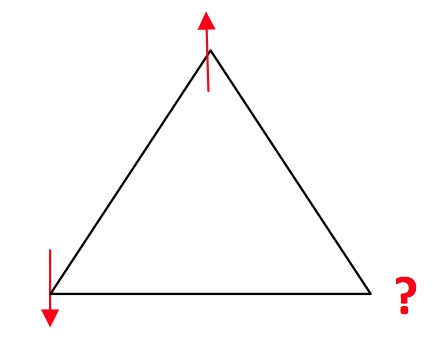
\includegraphics[scale=0.5]{images/frustration.jpg}
\caption{In the antiferromagnetic 2D Ising model on a triangular lattice there is no way one can orient the spins to minimize all interactions simultaneously.}
\label{fig:frustration}
\end{figure}

\subsection{The Ising Spin Glass}
In the previous section we concluded by introducing the concept of frustration through geometric frustration on a triangular lattice. There are however other ways to create frustrated systems and one of them is to introduce a new Hamiltonian

\begin{equation}
H=\sum\limits_{\left\langle i,j \right\rangle} J_{ij} S_{i} S_{j}
\end{equation}
where the coupling constants $J_{ij}$ are now a Gaussian distributed random numbers with mean zero and variance one. This Hamiltonian describes a class of disordered systems and we will focus on a subgroup of these called \emph{spin glasses} (SGs). What is special about SGs is the fact that they have a finite temperature disordered ground state. This means that below a critical temperature $T_c$ the disordered system will "freeze" with the spins in random positions determined by the particular set of couplings. However, depending on the dimension of the lattice there is a critical dimension below which no finite temperature glass phase exists\cite{almeida}.

The main objective when examining disordered system is often to determine the critical exponents and we will concern ourselves with one of these, namely the \emph{stiffness exponent} $\theta$. It can be obtained through the scaling ansatz

\begin{equation}
\Delta E \thicksim L^\theta
\label{eq:scaling}
\end{equation}
where $L$ is the system size and $\Delta E$ is the cost of a domain wall. We will use the tried and true P-AP method\cite{hartmann}\cite{carter} to calculate $\Delta E$ which can be outlined as follows:

\begin{enumerate}
\item Generate a random set of couplings and a random configuration of spins, i.e. a configuration at $T=\infty$, using periodic boundary conditions (PBCs).
\item Perform a quench by sequentially sweeping through the system and flip a spin if it is energetically favourable. Repeat until no more flips are accepted during a whole system sweep.
\item Calculate the energy of the spin configuration $E_{PBC}$ and perform a huge number of quenches with the same \emph{couplings} but random spin configurations. The lowest energy found in this way yields an approximate ground state energy.
\item Switch to anti-periodic boundary conditions (APBCs) by changing the sign of $J_{ij}$ along $x=L$ and repeat step 1-3 to obtain $E_{APBC}$.
\item The cost of a domain wall is now given by $\Delta E = \commutator{|E_{PBC}-E_{APBC}|}$, where $[...]$ means averaging over different sets of couplings.
\end{enumerate}
Using Eq. \eqref{eq:scaling} the stiffness exponent can now be obtained by calculating and plotting $\Delta E$ for different system sizes. The stiffness exponent is a measure of how the strength of systems couplings scale in the low temperature phase in a renormalization group sense. If the sign of $\theta$ is positive the system scales to strong couplings and conversely if the sign is negative the system scales to weak couplings and this is characteristic behaviour for SGs and the paramagnetic phase, respectively \cite{almeida}. What happens is that the system gets stuck in local minima and there will an energy barrier that needs to be crossed for the system to break out of this metastable state. The size of this energy barrier is determined by the stiffness exponent and thus in 2D the size of the energy barriers decrease with system size allowing and in 3D they increase.

As previously stated the objective of this project is to determine the stiffness exponent on a square lattice in two and three dimensions, using the algorithm for obtaining $\Delta E$ outlined above.

\section{Method}
\label{sec:method}
We start from a serial implementation which works as follows. Beginning at the first lattice site, the Hamiltonian is applied to the current spin and a spin-flip is evaluated and accepted if energetically favourable. This is done for every spin, one after the other. These lattice sweeps are repeated until there are no spins flips during a whole sweep. This is a rather trivial algorithm that is easily set up and run with a single thread on a conventional CPU using any given language. For this project we are provided with an implementation written in C, that executes the given algorithm for a 2D lattice. This we generalized to a serial version for a 3D lattice. However, the implementation of the serial code will not be subject to further discussion in this paper, but will rather serve as a reference point for data verification and performance comparison.

A first CUDA implementation of the code will be written for the 2D lattice using the serial version as reference. This implementation will already be written with focus on efficient parallelization. The CUDA 3D version will in turn be developed using the CUDA 2D version as basis. These first implementations are then enhanced with CUDA specific functions like error handling and device selection. The last enhancement will be an OpenMP version that uses several host threads in order to be able to utilize multiple GPUs for calculations.

\subsection{NVIDIA GPU Architecture}
NVIDIA Fermi or Kepler architecture GPUs consist of several streaming multiprocessors (SMs) which contain the so called CUDA cores (c.f. figure \ref{fig:fermi_sm}). Typical numbers are 16 SMs with 32 CUDA cores each (512 cores in total) for the Fermi architecture. And 14 SMs with 192 CUDA cores each (2688 cores in total) for its successor, the Kepler architecture. Compared to a CPU core these CUDA cores are rather simple. They can execute one instruction (floating point or integer) for a thread per clock cycle. All cores in a SM have access to a small amount of shared memory (typical 16 or 48 KiB, the 64 KiB in figure \ref{fig:fermi_sm} are shared memory and L1 cache combined). This memory has low latency but can only be accessed by threads executed by the same SM. All SMs have access to the global GPU memory which is nowadays several GiB in size.

\begin{figure}
\centering
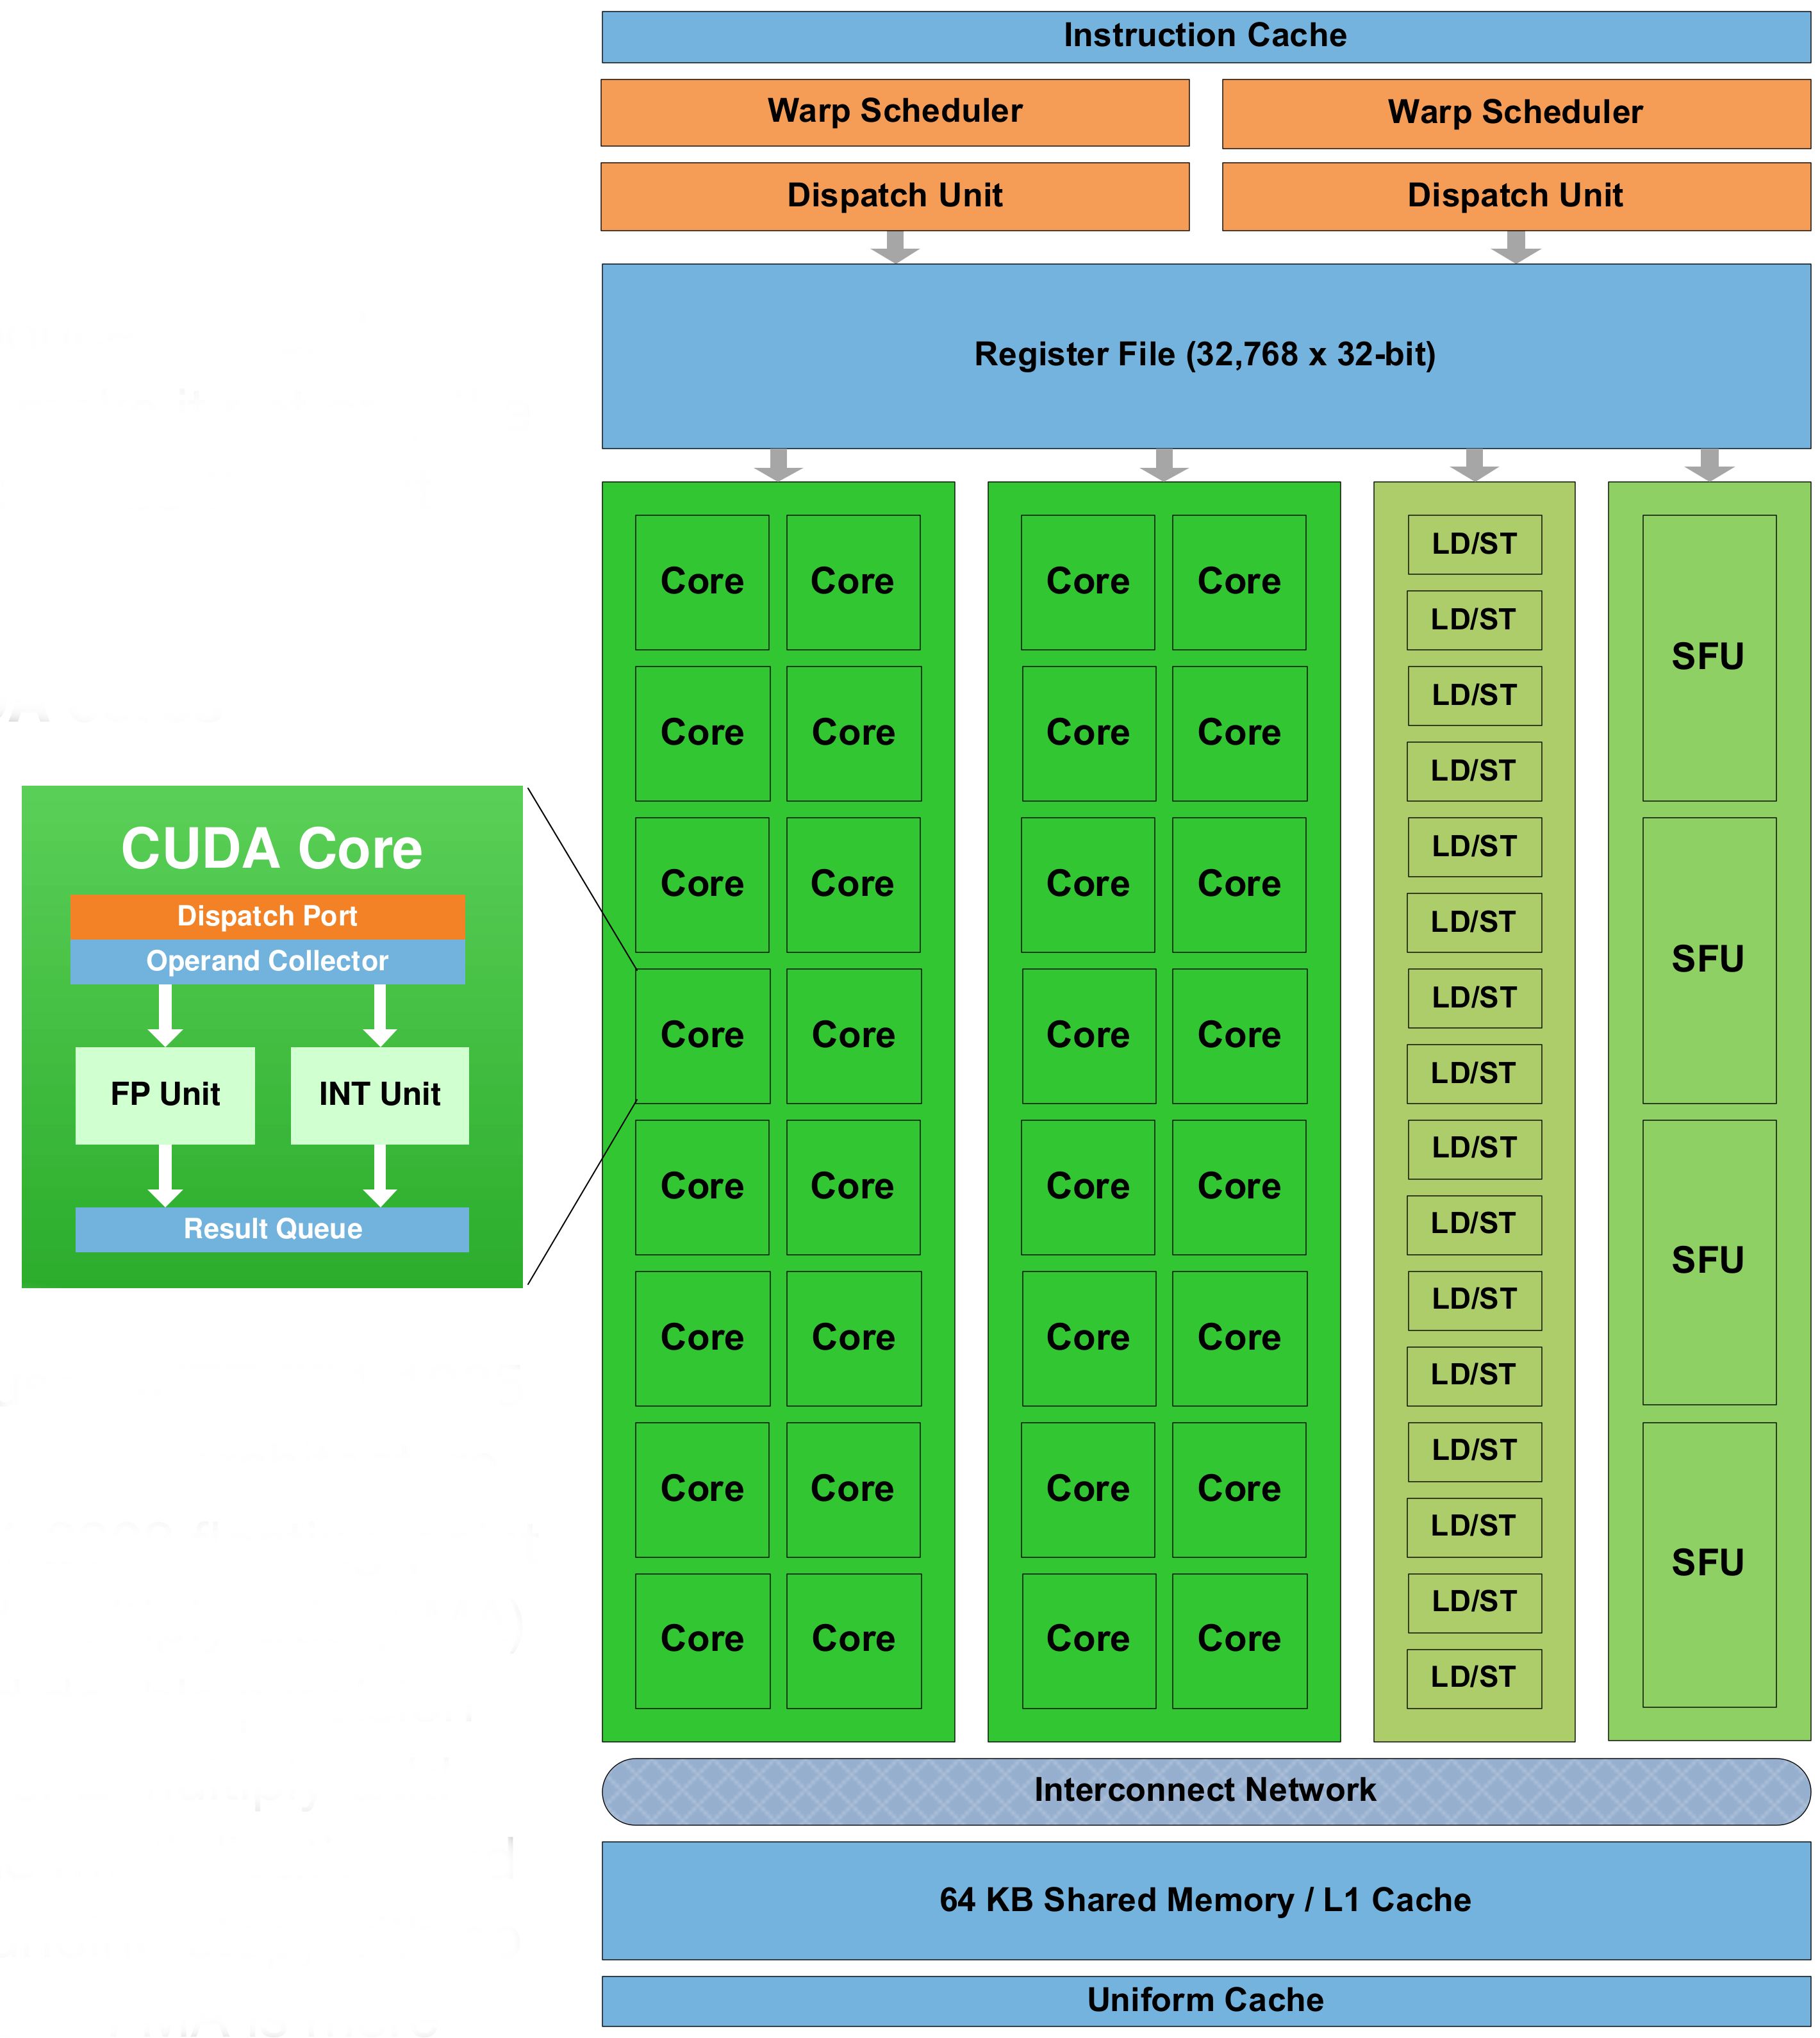
\includegraphics[width=.8\linewidth]{images/fermi_sm.png}
\caption{Schematic of a streaming multiprocessor (NVIDIA Fermi architecture)\cite{gpu_nvidia_fermi}.}
\label{fig:fermi_sm}
\end{figure}

\subsection{CUDA Programming Model}
A CUDA program can consist of \textsc{C}, \textsc{C++}, \textsc{Fortran} (more languages are supported) code with parts that are executed on the host CPU and parts that are executed on the GPU (the s.c. kernels). Due to the GPU architecture these kernels are launched in grids of blocks of threads. Depending on the hardware each block can contain up to 512 or 1024 threads. All threads within a block have access to the same shared memory. For execution on the SMs threads are grouped in s.c. warps of 32 threads.

To organize threads in CUDA one can use synchronization barriers and each thread has variables that contain thread and block indices. It is also important to note that CPU and GPU do not share the same memory address space, hence data has to be copied from/to host memory to/from GPU memory for processing. Even though, with CUDA version 6 one does not have to take care of this explicitly any more it is still an important thing to keep in mind in order to write efficient code.


\subsection{CUDA Implementation}
To be able to parallelize any problem in general one is required to split it up into isolated tasks, that in turn can be distributed to the available computational units. If one fails to accomplish isolated calculations a phenomenon known as race conditions will result in non-deterministic calculations. This essentially emerges from the fact that individual computational units execute code in an undefined order. Here we present an approach to surmount this issue in the 2D and 3D case similar to that presented by M. Weigel and T. Yavors \cite{gpu_mc_spins}.

\subsubsection{Two Dimensions}
By placing a checker pattern over the 2D grid of spins (,figure \ref{fig:checker_grid}) the system is divided into black and white tiles. Notice that there are no adjacent tiles of the same color and hence there are no interactions between tiles of the same color. Therefore each set of black or white tiles is individually isolated and thus suitable for parallel computing. One colour set of tiles will be processed while the others remain unchanged. After the first set of tiles is completed, shared and global memory is synchronized and the remaining tiles are processed.

Each tile in the set will be designated for one CUDA block. To avoid repeated access to global memory all spins of a tile should be copied to shared memory before starting the actual calculation. Each given tile will interact with the nearest neighbour spins around it, hence it is necessary to bring these spins and their corresponding couplings into shared memory too. Referred to as ghost couplings and spins, these are shown respectively as dashed lines and blue blobs in figure \ref{fig:gost_cells} for a tile of $2\times2$.


\begin{figure}
\centering
\begin{minipage}{.65\textwidth}
  \centering
  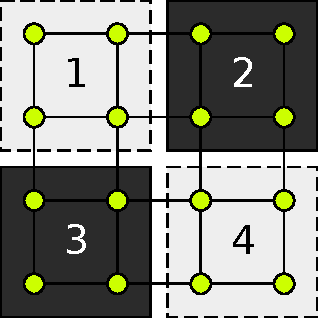
\includegraphics[width=.5\linewidth]{images/4x4.pdf}
  \caption{The two groups of tiles are marked with black and white squares. Here the spins in tile 1 and 4 can be processed in parallel while 2 and 3 remain unchanged and vice-versa.}
  \label{fig:checker_grid}
\end{minipage}
\hspace{0.05\linewidth}
\begin{minipage}{.25\textwidth}
  \centering
  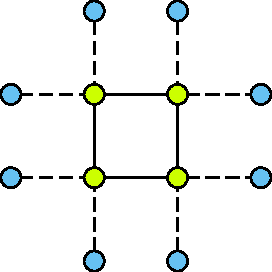
\includegraphics[width=1\linewidth]{images/2D_ghosts.pdf}
  \captionof{figure}{A tile including ghost cells.}
  \label{fig:gost_cells}
\end{minipage}
\end{figure}


It is further recognized that ghost spins will have to be selected with the periodic boundary condition in mind. Hence, the indices of for instance the neighbouring spins in the two directions along the x-axis will be
\begin{align*}
x_+&=(x_c+1)\; \text{mod} \; L \;, \\
x_-&=(x_c-1+L) \; \text{mod} \; L \;.
\end{align*}
Here $x_+$ and $x_-$ are the indices of the neighbouring spins along the positive and negative direction of the x-axis, $x_c$ is the index of the current spin, $L$ the side of the global system and "mod" signifies the modulus operator.

The number of CUDA blocks is only half the amount of tiles since only one tile colour can be processed in parallel at a time. In the example shown in figure \ref{fig:checker_grid} there are two CUDA blocks for calculation and when they are finished the white tiles are submitted. This is done row-wise, where a group of a black and a white tile are sequentially sent for calculation. The first tile of the first row is chosen to be white, then in the second row the second tile is instead white. This is achieved in 2D by alternating between these selection-modes using the condition 
\begin{equation}
b_y\; \text{mod} \; 2 == 0 \;,
\label{eq:sele_mode_2d}
\end{equation}
where $b_y$ is the block row index. This condition will yield \textsc{true} if $b_y$ is even and \textsc{false} otherwise.

The spins will be processed by threads inside each block. These threads have access to the same shared memory and will begin to populate it with data picked from global memory. Here the number of spins processed by each thread is fixed to 2. Shown for the $2\times2$ block in figure \ref{fig:2D_threads} each thread will process one spin at a time. To avoid race conditions a synchronization is performed in between the two spin flips by each thread. Thus, the spins processed in parallel are marked as red and green respectively for each set. The selection of the first or the second spin to be handled first by each thread is based on the same condition as in \ref{eq:sele_mode_2d}.
 
This division into 2 spins per thread will imply a divisibility by 2 for the block size. And because we have two tiles that are processed after each other the system size will have to be divisible by 2 times the block size. For the sake of simplicity we use system sizes of $4\times4$, $8\times8$, $16\times16$, $32\times32$ and so on.

Multi-dimensional arrays are avoided even though it is more convenient from the programming point of view. Especially since CUDA provides functions for handling this kind of setup. The reason they are avoided is foremost since they introduce extra overhead in the form of an extra memory lookup during access and in the form of more expensive allocation and population during initialization and transfer between host and device.

The access is instead solved by the utilization of an arithmetic operation where the location in memory is calculated before access using $x + y \times L$, where $x$ is the column index, $y$ is the row index and $L$ is the column count of each row.

\begin{figure}
\centering
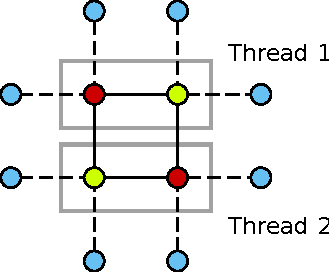
\includegraphics[width=.4\linewidth]{images/2D_threads.pdf}
\caption{Thread division in each block. Non-interacting spins are grouped in red and green.}
\label{fig:2D_threads}
\end{figure}


\subsubsection{Three Dimensions}
In three dimensions basically the same approach is employed. However, there is an extra set of couplings along the new direction and all the system quantities are added an extra dimension. That is the three sets of couplings and the spins. 

Furthermore, the selection-mode for starting with black or white tiles at each row is instead of the condition \ref{eq:sele_mode_2d} chosen based on
\begin{equation}
(b_y + b_z)\; \text{mod} \; 2 == 0 \;,
\end{equation}
where $b_y$ and $b_z$ are the row and depth indices of the blocks, respectively. 

In addition to this another key difference compared to the 2D version is the calculation of the memory index. We need to include the depth index $z$ as well, yielding $x + y \times L + z \times L^2$.


\subsection{Performance Considerations}
Since access to global memory has high latency compared to shared memory it is in general a good idea to copy all data that threads in a block need from global to shared memory before processing it. This will be done in our code.

In our implementation we will stick to the random number generator host code in order to get directly comparable results with the sequential implementation. The drawback of this is that we have to create our spin and coupling configurations in host memory and then copy it to the device before we can start the calculation. Especially for larger systems the time of this data transfer becomes noticeable. But at least this is a way to share work between the GPU and CPU. For cases where the CPU is slowing down the GPU one could use the \href{http://docs.nvidia.com/cuda/curand/index.html}{cuRAND} library to create random numbers directly on the GPU.

We want to be able to use multiple GPUs for our calculations. A straightforward way to do this with our code is to use OpenMP to create one host thread per GPU and divide the loop over random spin sets amongst several GPUs. One could also use OpenMP to further parallelize the initialization of the spin sets that happen on the CPU. But because OpenMP creates overhead and most of the calculation time is spent on the GPU this does not seem promising.

In order to get good GPU utilization we will have to keep all SMs (and CUDA cores) occupied. If we assume 16 SMs and 500 to 2000 cores it is clear that for smaller system sizes our rather simple implementation will not be able to create enough threads to do that.

Possibilities to reduce or circumvent aforementioned drawbacks will be discussed in section \ref{sec:discussion_gpualgo}.

\section{Results}
\label{sec:results}
The simulation data obtained through the method and algorithms explained in the previous sections will be displayed and explained in this section.

\subsection{The Stiffness Exponent}
In Fig. \ref{fig:E_2D_large} and \ref{fig:E_3D_large} we can see the square of the domain wall energy in two and three dimensions plotted versus the system size for an increasing number of quenches. Fig. \ref{fig:E_2D_small} and \ref{fig:E_3D_small} are the same graphs but focused on the interval where the best accuracy is achieved. Tab. \ref{tab:stiffness_exponent} contains all values obtained for the stiffness exponent from the different curves. These values are obtained by making a least square fit for the points $L=4$ and $L=8$ since the domain wall energy is rapidly growing for larger system sizes. In table Tab. \ref{tab:couplings_2D} and \ref{tab:couplings_3D} are the number of disorders couplings used to obtain statistical accuracy for different system sizes and number of quenches. The cost of a domain wall as well as the standard deviation is calculated using these values and is reflected by the error bars in Fig. \ref{fig:E_2D_large}, \ref{fig:E_3D_large}, \ref{fig:E_2D_small} and \ref{fig:E_3D_small}.

\begin{table}[h]
\centering
  \begin{tabular}{| c | c | c |}
    \hline
    $N_{quenches}$ & $\theta_{2D}$ & $\theta_{3D}$ \\ \hline
    $10^2$ & $0.4288$ & $1.4310$ \\ \hline
    $10^3$ & $0.1293$ & $1.4116$ \\ \hline
    $10^4$ & $-0.2404$ & $1.2678$ \\ \hline
    $10^6$ & $-0.6394$ & $1.4897$ \\ \hline
    $10^8$ & $-1.2623$ & $0.8337$ \\ \hline
    Reference & $-0.289$ & $0.225$ \\ \hline
  \end{tabular}
  \caption{The value of the stiffness exponent obtained by least square fit from the two smallest system sizes $L=4,8$ in 2D and 3D.}
  \label{tab:stiffness_exponent}
\end{table}

\begin{table}[h]
\centering
  \begin{tabular}{| c | c | c | c | c | c | c |}
    \hline
    N/L & 4 & 8 & 16 & 32 & 64 & 128 \\ \hline
	2 & 1000 & 1000 & 1000 & 1000 & 1000 & 1050 \\ \hline
	3 & 1000 & 1000 & 1000 & 1000 & 1000 & 1050 \\ \hline
	4 & 1000 & 1000 & 1000 & 200 & 100 & 1050 \\ \hline
	6 & 100 & 100 & 100 & 200 & 100 & 75 \\ \hline
	8 & 10 & 10 & 10 & 5 & 3 & 2 \\ \hline
  \end{tabular}
  \caption{The number of different sets of disordered couplings used to obtain the average groundstate for different system sizes and number of quenches in 2D.}
  \label{tab:couplings_2D}
\end{table}

\begin{table}[h]
\centering
  \begin{tabular}{| c | c | c | c | c |}
    \hline
    N/L & 4 & 8 & 16 & 32 \\ \hline
	2 & 1000 & 1000 & 1000 & 1000 \\ \hline
	3 & 1000 & 1000 & 1000 & 1000 \\ \hline
	4 & 100 & 100 & 100 & 100 \\ \hline
	6 & 100 & 100 & 100 & 80 \\ \hline
	8 & 38 & 10 & 16 & 3 \\ \hline
  \end{tabular}
  \caption{The number of different sets of disordered couplings used to obtain the average groundstate for different system sizes and number of quenches in 3D.}
  \label{tab:couplings_3D}
\end{table}

\begin{figure}
\centering
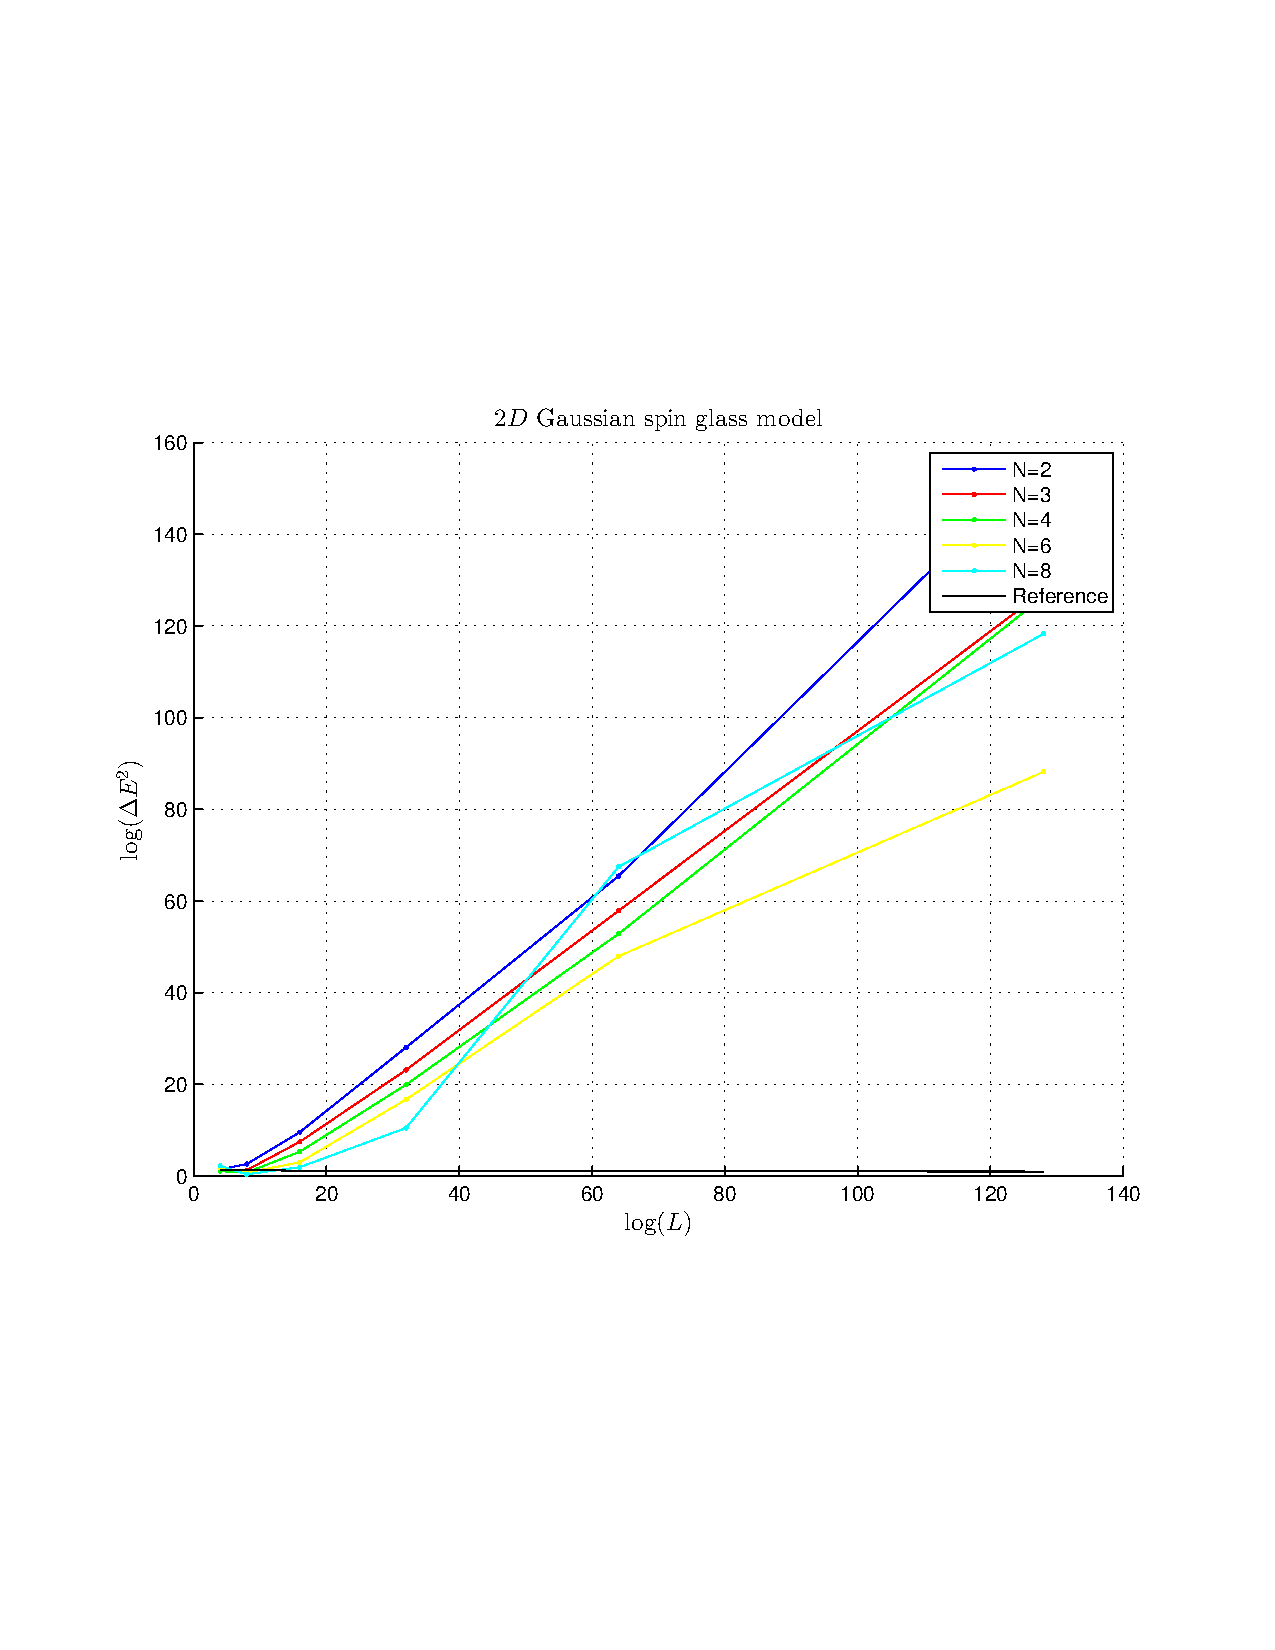
\includegraphics[width=\textwidth]{images/spinglass2D_large.pdf}
\caption{The square of the domain wall energy $\Delta E ^ 2$ as a function of system size $L$ for different number of quenches in two dimensions. The black line is the reference value for the stiffness exponent $\theta=-0.289$.}
\label{fig:E_2D_large}
\end{figure}

\begin{figure}
\centering
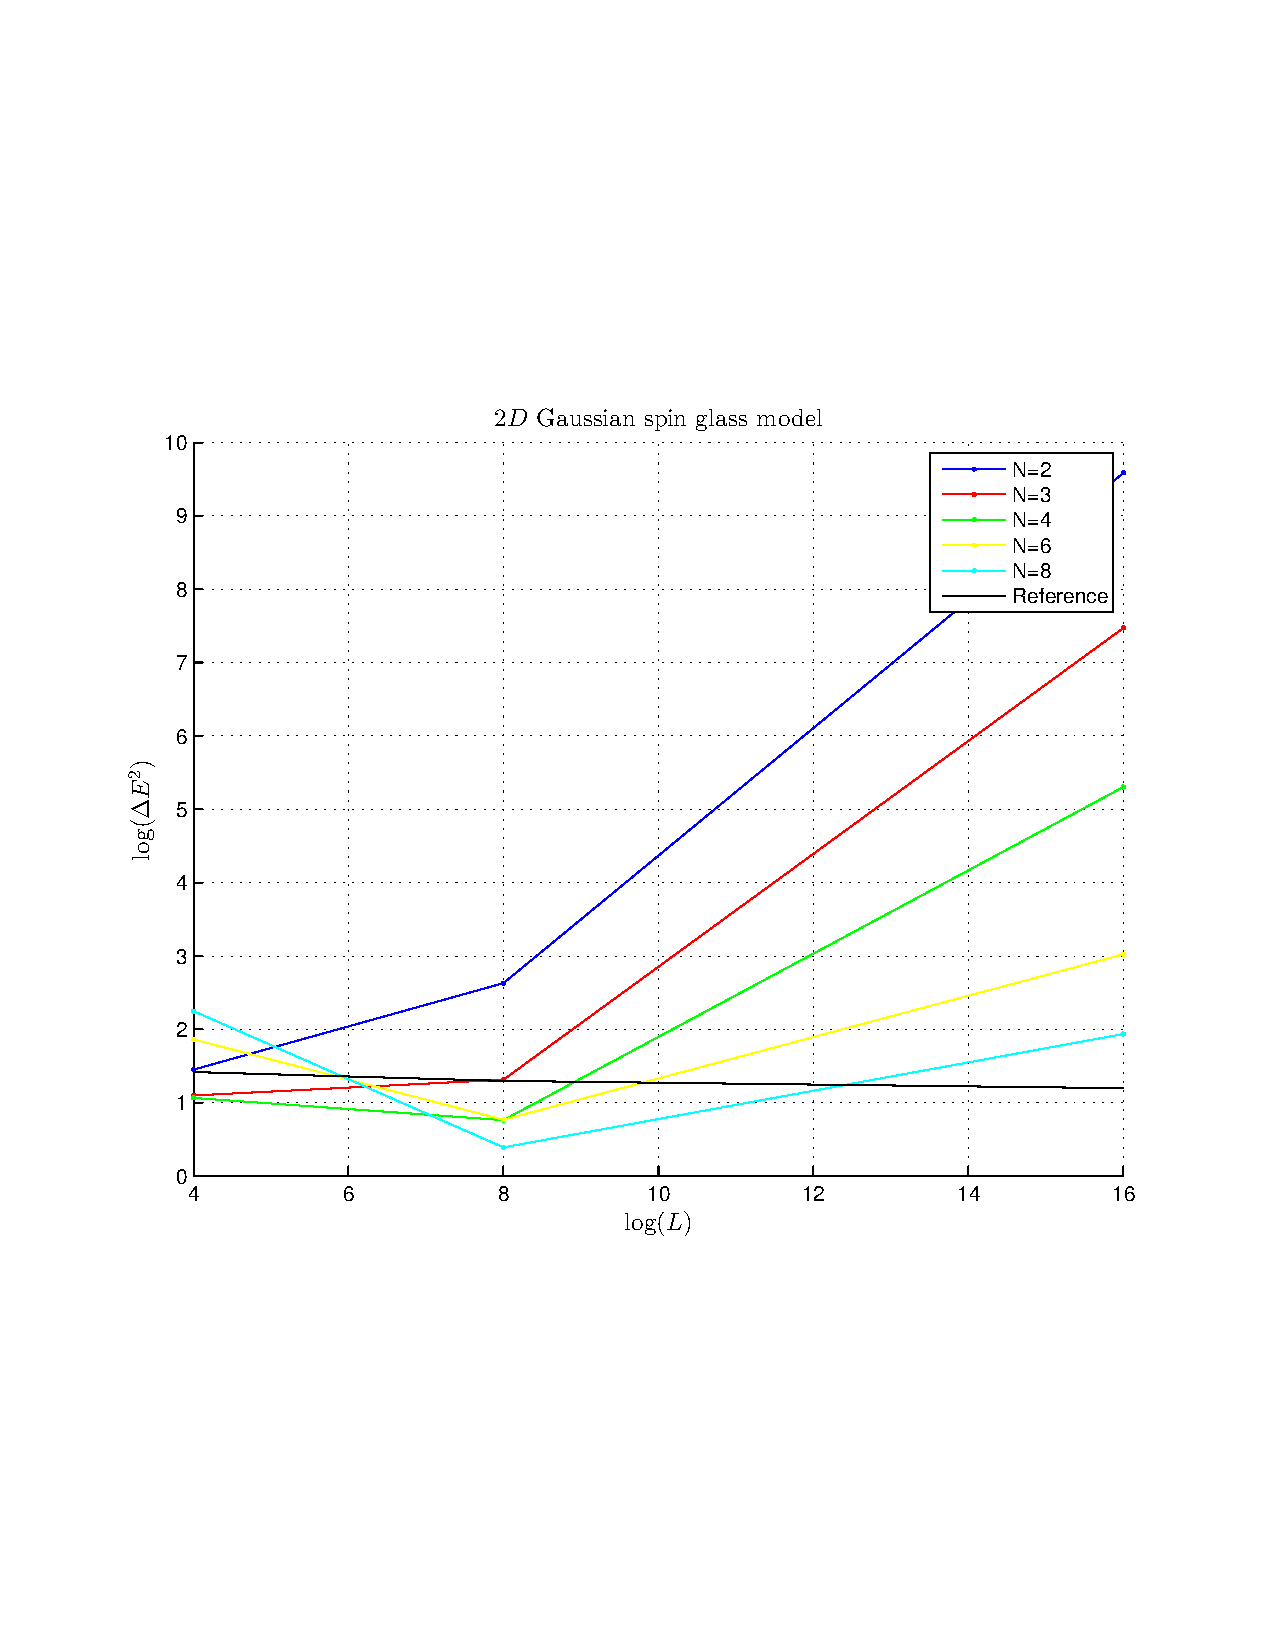
\includegraphics[width=\textwidth]{images/spinglass2D_small.pdf}
\caption{The square of the domain wall energy $\Delta E ^ 2$ as a function of system size $L$ for different number of quenches in two dimensions. The black line is the reference value for the stiffness exponent $\theta=-0.289$.}
\label{fig:E_2D_small}
\end{figure}

\begin{figure}
\centering
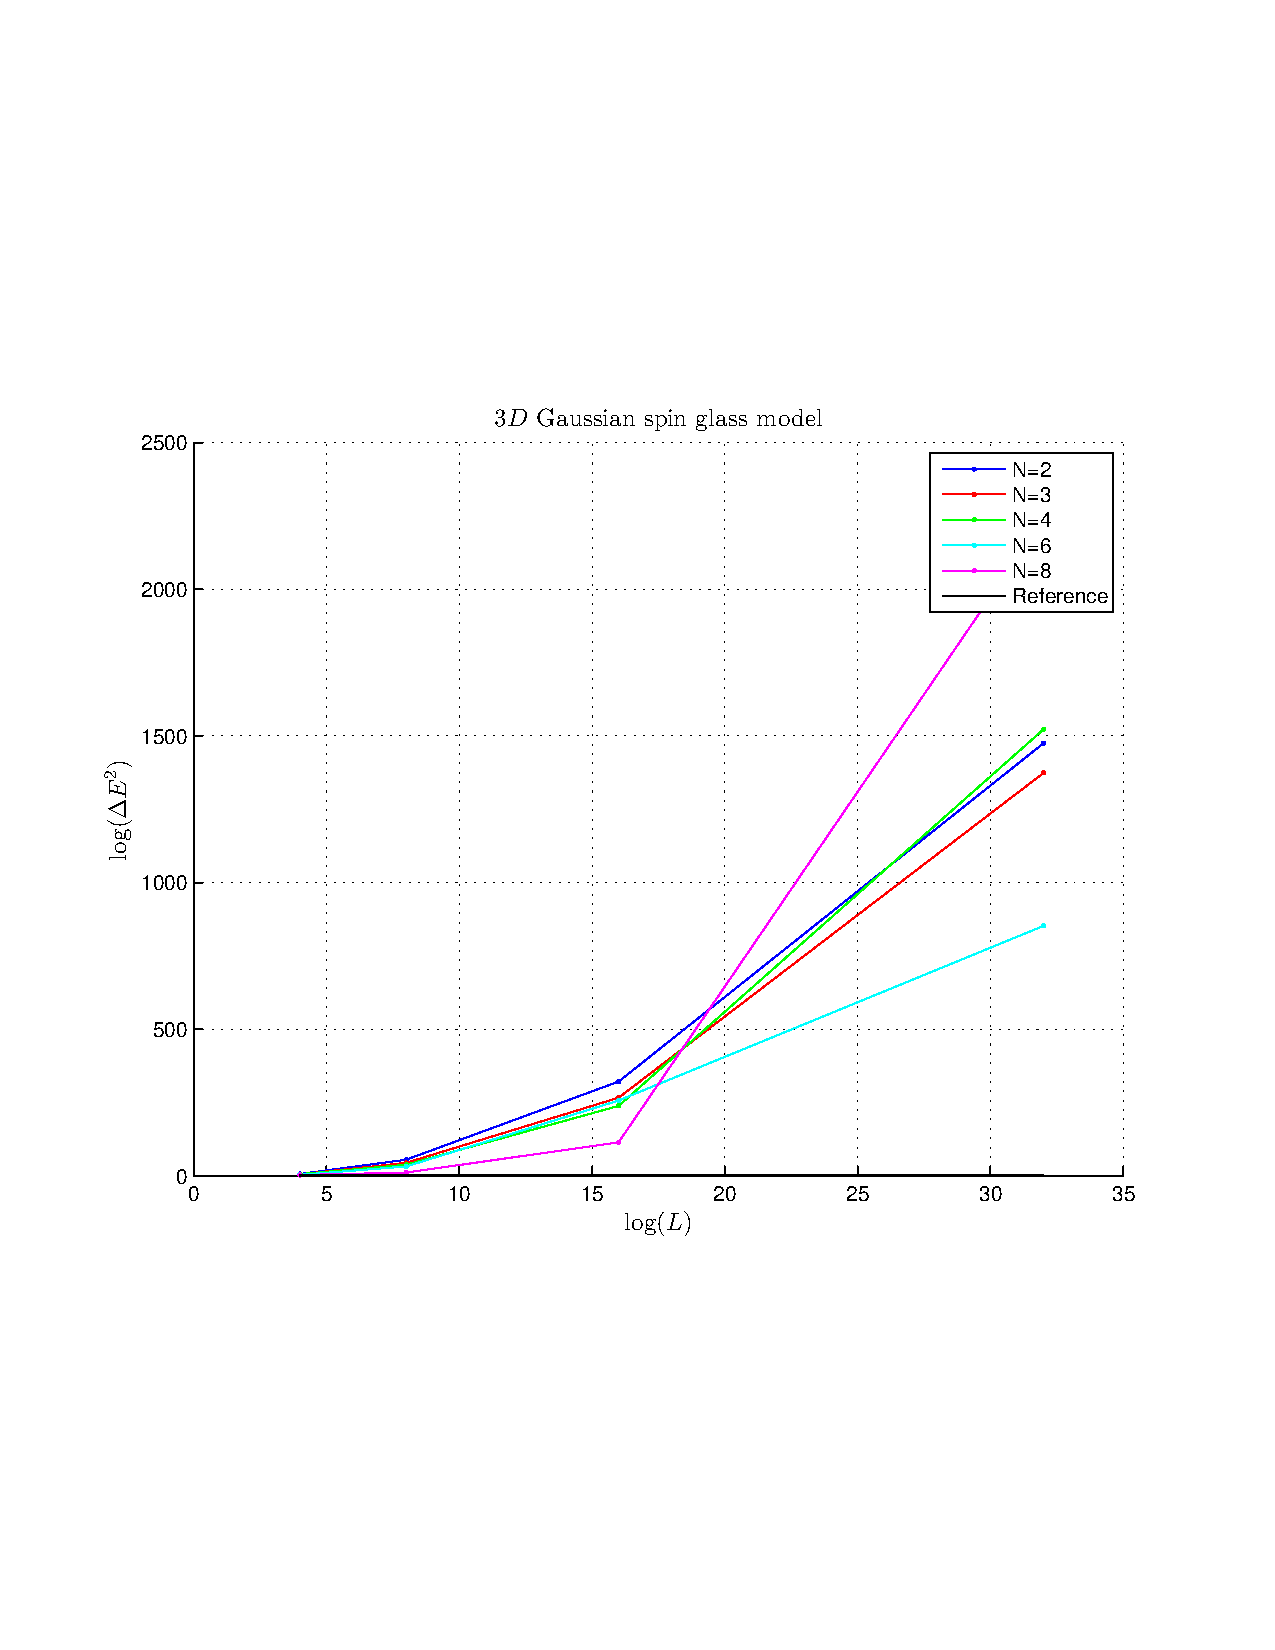
\includegraphics[width=\textwidth]{images/spinglass3D_large.pdf}
\caption{The square of the domain wall energy $\Delta E ^ 2$ as a function of system size $L$ for different number of quenches in three dimensions. The black line is the reference value of $\theta=0.225$.}
\label{fig:E_3D_large}
\end{figure}

\begin{figure}
\centering
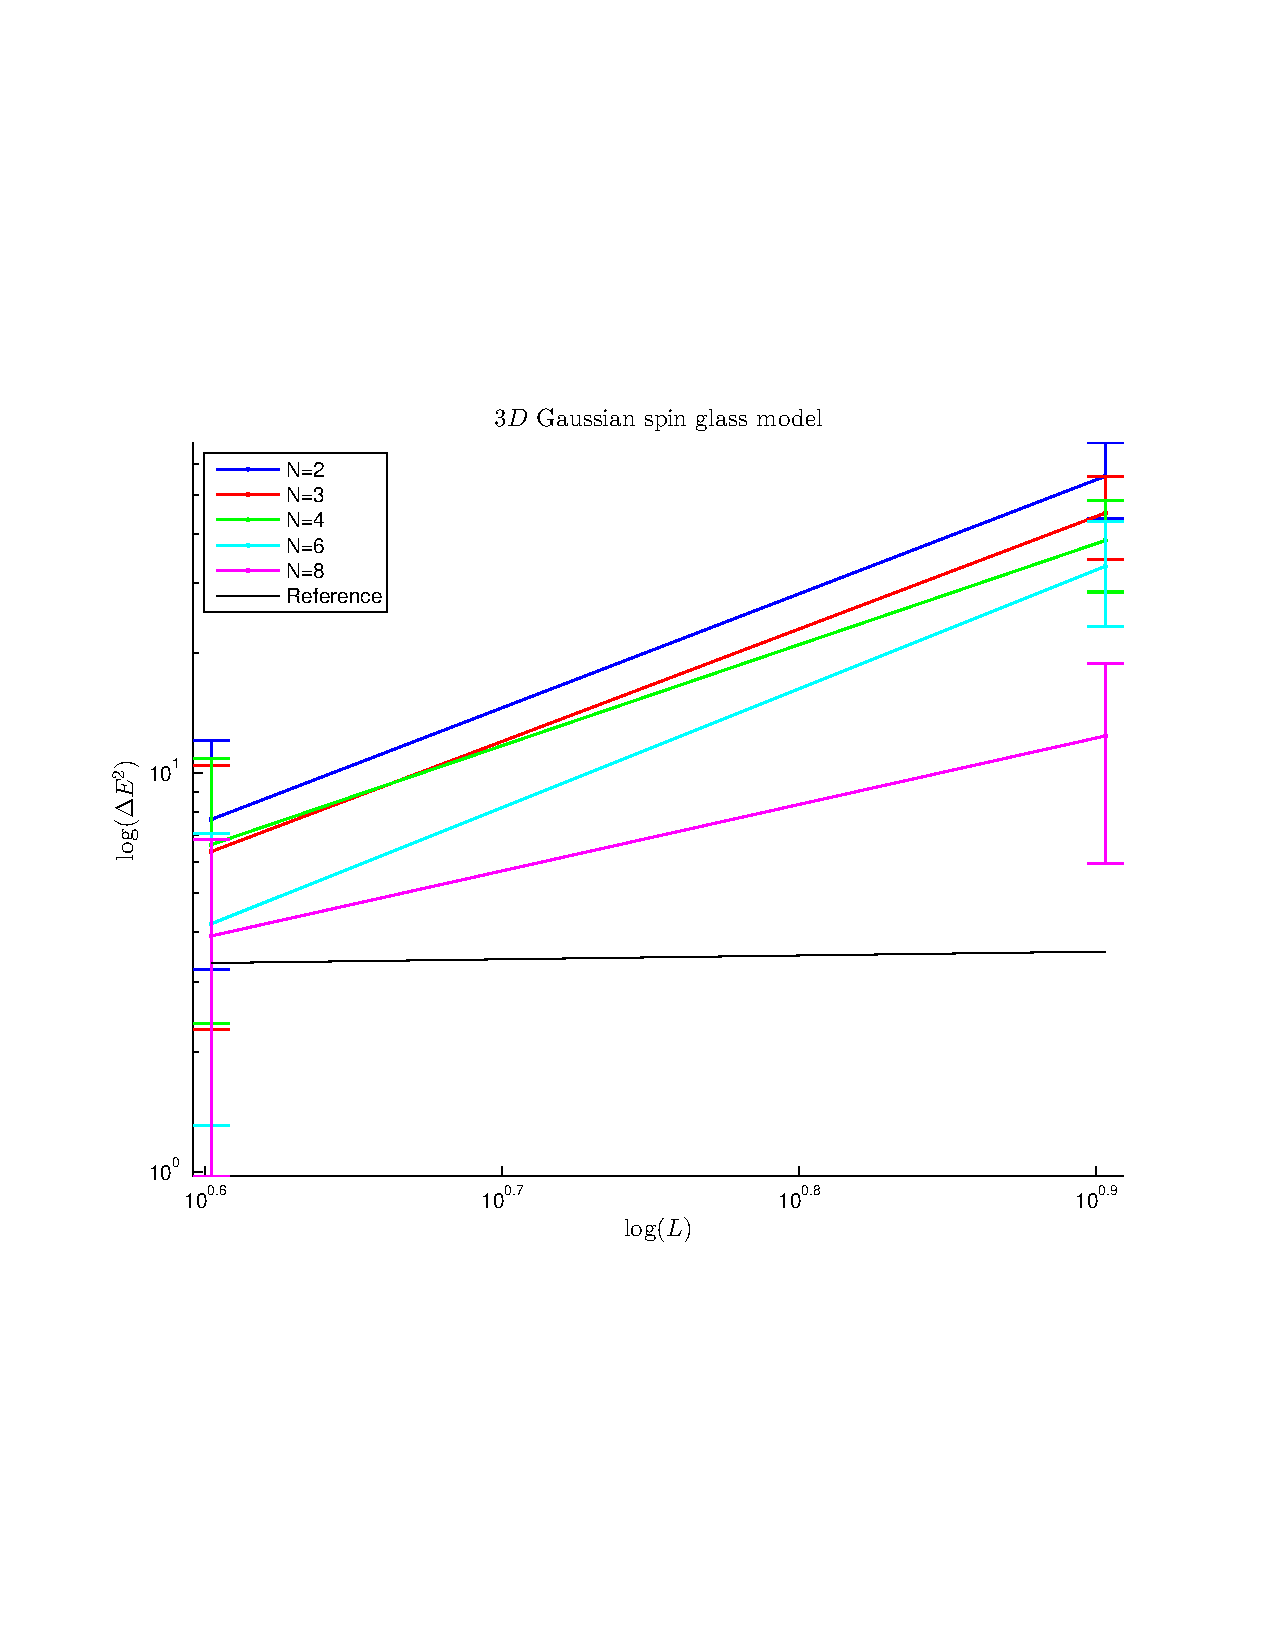
\includegraphics[width=\textwidth]{images/spinglass3D_small.pdf}
\caption{The square of the domain wall energy $\Delta E ^ 2$ as a function of system size $L$ for different number of quenches in three dimensions. The black line is the reference value of $\theta=0.225$.}
\label{fig:E_3D_small}
\end{figure}

\subsection{GPU-Algorithm Performance}
As expected, for small system sizes our code does not create enough parallelism and can therefore not fully utilize the GPU. Figure \ref{fig:perf_flips} shows the achieved spin updates per nanosecond for different system sizes in 2D and 3D. First we can see that our OpenMP code with one thread is not slower than the code without OpenMP. We can also see that our approach to use multiple GPUs (with one OpenMP thread per GPU) is promising. The per-GPU performance with OpenMP threads is not more than $10\%$ lower than the reference performance of a single GPU without OpenMP. For the largest tested system size (512 in 3D) measurements become somewhat unstable because of the long transfer times to/from GPU memory.

\begin{figure}
\centering
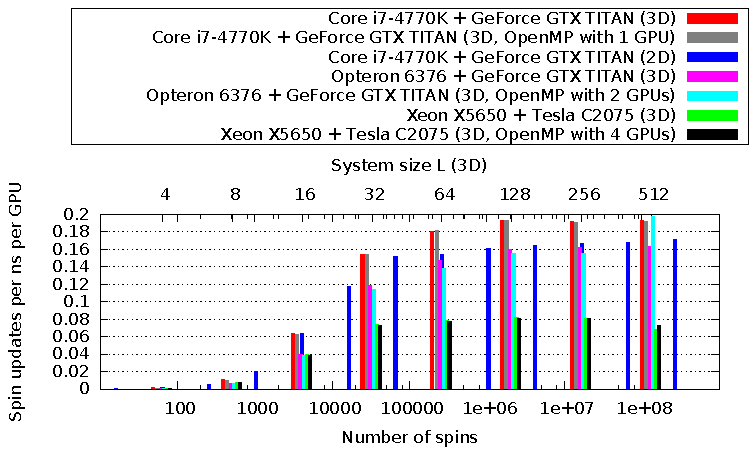
\includegraphics[width=\textwidth]{images/perf_flips.pdf}
\caption{Spin updates per nanosecond for different system sizes to compare single GPU vs. multiple GPUs with OpenMP and different CPUs.}
\label{fig:perf_flips}
\end{figure}

If we compare the runs with GeForce GTX TITAN GPUs on different computers we also see that the host CPU influences the performance to some extend. We tried if it was possible to mitigate this by executing the host code with multiple OpenMP threads but that did not help, in fact performance went down. In our case apparently an AMD Opteron with 2.3 GHz clock speed can not get full performance out of a high-end GeForce GTX TITAN GPU. An Intel Core i7 with 3.5 GHz clock speed has an overall faster subsystem that manages to tax the GPU better.

Figure \ref{fig:perf_times} shows typical execution times for various system sizes in 2D and 3D. Because performance of our code is not constant for varying system sizes it is not a simple $L^2$ or $L^3$ dependency. Another factor is that the larger the system, the more lattice sweeps are needed to reach a minimum. Table \ref{tab:avg_sweeps} shows the average number of sweeps necessary to reach a minimum for different system sizes.

\begin{figure}
\centering
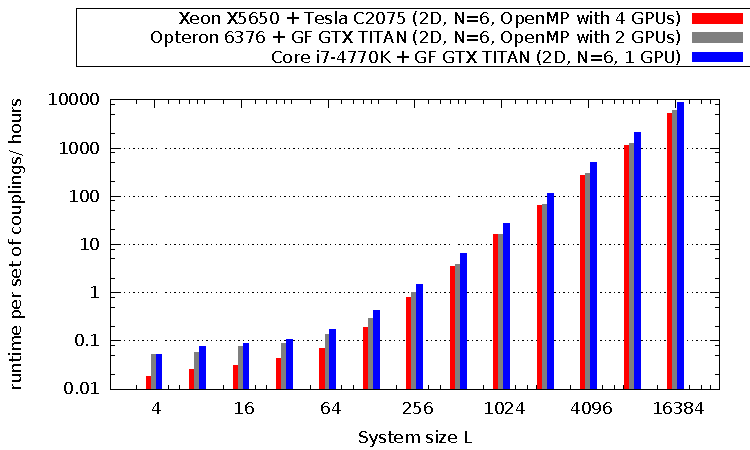
\includegraphics[width=0.65\textwidth]{images/perf_time2d.pdf}
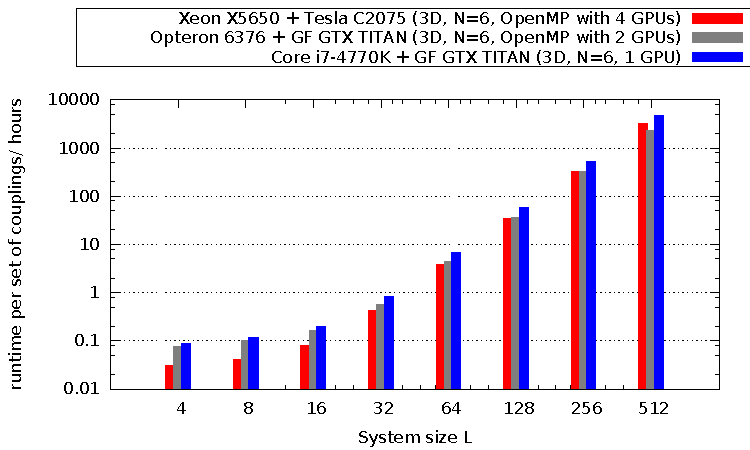
\includegraphics[width=0.65\textwidth]{images/perf_time3d.pdf}
\caption{Typical run times for various system sizes in 2D and 3D for N=6 ($10^6$ spin sets).}
\label{fig:perf_times}
\end{figure}

\begin{table}
\centering
  \begin{tabular}{| c | c | c | c | c | c | c | c | c | c | c | c | c | c |}
    \hline
    L & 4 & 8 & 16 & 32 & 64 & 128 & 256 & 512 & 1024 & 2048 & 4096 & 8192 & 16384 \\ \hline
	$n_{sweeps}$, 2D & 3.2 & 4.9 &  6.6 &  8.3 &  9.3 & 10.7 & 12.7 & 13.6 & 15.0 & 16.3 & 17.9 & 19.2 & 20.5 \\ \hline
	$n_{sweeps}$, 3D & 5.8 & 8.2 & 11.0 & 13.8 & 16.4 & 19.2 & 21.9 & 24.4 &      &      &      &      &      \\ \hline
  \end{tabular}
  \caption{Average number of lattice sweeps for different system sizes until a minimum is reached.}
  \label{tab:avg_sweeps}
\end{table}


\section{Discussion}
\label{sec:discussion}
In this section we will discuss both the physical results and the performance of our algorithm.

\subsection{The Stiffness Exponent}
Calculating the stiffness exponent is, to say the least, a time consuming task requiring huge amounts of computations. As displayed in Fig. \ref{fig:E_2D_large} and \ref{fig:E_3D_large} the number of quenches necessary to obtain a decent approximation the ground state rapidly increases and on top of that, the time to perform each quench increases with the system size. This can be seen by observing that $(\Delta E)^2$ rapidly diverges from the expected result for a low number of quenches. This reflects the nature of the SGs with huge numbers of metastable states and the difficulty to find an approximate ground state. One has to start from increasingly many initial spin configurations in order to find a few where you do not get stuck in a local minimum. 

From Tab. \ref{tab:stiffness_exponent} we can see that the best values obtained are $\theta_{2D}=-0.24$ for $10^4$ quenches and $\theta_{3D}=0.83$ for $10^8$ quenches in two and three dimensions respectively. In two dimensions this is a quite good value and in three dimension it is at least decent. To obtain better values one would primary need to average over more couplings and secondary go to a higher number of quenches.

The only upside with this extremely complex problem is the fact that it is parallelizable and thus well suited for computing on a GPU.

\subsection{GPU-Algorithm Performance}
\label{sec:discussion_gpualgo}

One  approach to minimize this influence of the host CPU could be the use of cuRAND to generate random numbers on the GPU. One could also try to hide host to device memory copy times by preparing and copying new data while the GPU is processing the current data set. Performance for larger systems is good, therefore to increase performance for small system sizes the following approach might be promising. Instead of generating small arrays for spins and couplings one could create multiple configurations at once embedded in a larger array that is sent to the GPU for processing. It is not entirely trivial because of boundary conditions but not too complex either.


\section{Conclusion}
\label{sec:conclusions}
To summarize, we have calculated the stiffness exponent $\theta$ for the nearest-neighbour interaction Gaussian Ising spin glass on a square lattice in two and three dimension using the scaling ansatz $\Delta E \thicksim L^\theta$. The domain wall energy $\Delta E$ was calculated using the P-AP method. The value for the stiffness exponent was obtained by curve fitting in a least square sense and the best estimate is found to be $\theta_{2D}=-0.24$ for $10^4$ quenches and $\theta_{3D}=0.83$ for $10^8$ quenches in two and three dimensions respectively. Since $\theta_{2D}<0$ we conclude that there exists no finite temperature glass phase in two dimensions, however in three dimensions $\theta_{3D}>0$ implies that a there is indeed a finite temperature glass phase in agreement with other simulations as well as experiments\cite{hartmann}\cite{fisher}\cite{carter}. 

The implementation of the model was an optimized GPU-accelerated algorithm using CUDA which had great performance and showed great promise for future research.

\pagebreak
\section*{Appendix: Simulation Code (3D, OpenMP)}
\lstinputlisting[language=C++]{spinglass3d_omp.cu}

\pagebreak

\begin{thebibliography}{100}

\bibitem{onsager}
\textit{Crystal Statistics I. A Two-Dimensional Model with an Order-Disorder Transition} \\
L.Onsager \\
Phys. Rev. 65, 117, (1943)

\bibitem{almeida}
\textit{Chaos and stiffness exponents for short-range Gaussian Ising spin glasses} \\
Sebasti\~{a}o T O Almeida, Evaldo M F Curado andFernando D Nobre \\
J. Stat. Mech (2013)

\bibitem{hartmann}
\textit{Stiffness exponent of two-dimensional Ising spin glasses for nonperiodic boundary conditions using aspect-ratio scaling} \\
Phys. Rev. B 66, 224401 - Published 4 December 2002 \\
Alexander K. Hartmann, Alan J. Bray, A. C. Carter, M. A. Moore, and A. P. Young

\bibitem{fisher}
\textit{Theory of Random Magnets} \\
DS Fisher, GM Grinstein, A Khurana \\
Physics Today, 1988 

\bibitem{carter}
\textit{Aspect-Ratio Scaling and The Stiffness Exponent $\theta$ for Ising Spin Glasses} \\
A. C. Carter, A. J. Bray, M. A. Moore (January 4, 2014) \\
http://arxiv.org/pdf/cond-mat/0108050.pdf

\bibitem{nishimori}
\textit{Statistical Physics of Spin Glasses and Information Processing: An Introduction.} \\
Nishimori, Hidetoshi (2001). \\
Oxford: Oxford University Press. p. 243. ISBN 9780198509400.

\bibitem{gpu_mc_spins}
\textit{GPU accelerated Monte Carlo simulations of lattice spin models} \\
M. Weigel, T. Yavors. \\
Physics Procedia, \textbf{15} (2011)

\bibitem{gpu_nvidia_fermi}
\href{http://www.nvidia.com/content/pdf/fermi_white_papers/nvidia_fermi_compute_architecture_whitepaper.pdf}{\textit{Whitepaper -- NVIDIA's Next Generation CUDA Compute Architecture: Fermi}} \\
NVIDIA Corporation (2009)

\bibitem{gpu_nvidia_kepler}
\href{http://www.nvidia.com/content/pdf/kepler/NVIDIA-kepler-GK110-Architecture-Whitepaper.pdf}{\textit{Whitepaper -- NVIDIA's Next Generation CUDA Compute Architecture: Kepler GK110}} \\
NVIDIA Corporation (2012)


\end{thebibliography}
\end{document}
